\section{Experiments}

\subsection{Data}
\label{sec:data}

We briefly introduce our synthetic shape completion benchmarks, derived from ShapeNet \citep{Chang2015ARXIV} and ModelNet \citep{Wu2015CVPR} (\cf \figref{fig:data-shapenet-modelnet}), and our data preparation for KITTI \citep{Geiger2012CVPR} and \Kinect \citep{Yang2018ARXIVb} (\cf \figref{fig:data-kitti-yang}); \tabref{tab:data} summarizes key statistics \red{including the level of supervision computed as the fraction of observed voxels, \ie $\nicefrac{|\{x_{n,i} \neq \uk\}|}{HWD}$, averaged over observations $x_n$.}

\boldparagraph{ShapeNet}
%
We utilize the truncated SDF (TSDF) fusion approach of \cite{Riegler2017THREEDV} to obtain watertight versions of the provided car shapes allowing to reliably and efficiently compute occupancy grids and SDFs. Specifically, we use $100$ depth maps of $640 \ntimes 640$ pixels resolution, distributed uniformly on the sphere around the shape, and perform TSDF fusion at a resolution of $256^3$ voxels. Detailed watertight meshes, without inner structures, can then be extracted using marching cubes \citep{Lorensen1987SIGGRAPH} and simplified to $5\text{k}$ faces using MeshLab's quadratic simplification algorithm \citep{Cignoni2008EICC}, see \figref{fig:data-shapenet-modelnet-a} to \subref{fig:data-shapenet-modelnet-c}. Finally, we manually selected $220$ shapes from this collection, removing exotic cars, unwanted configurations, or shapes with large holes (\eg, missing floors or open windows).

The shapes are splitted into $|\mathcal{Y}| = 100$ reference shapes, $|\mathcal{Y}^*| = 100$ shapes for training the inference model, and $20$ test shapes. We randomly perturb rotation and scaling to obtain $5$ variants of each shape, voxelize them using triangle-voxel intersections and subsequently ``fill'' the obtained volumes using a connected components algorithm \citep{Jones2001}. For computing SDFs we use SDFGen\footnote{\url{https://github.com/christopherbatty/SDFGen}.}. We use three different resolutions: $H \ntimes W \ntimes D = 24 \ntimes 54 \ntimes 24$, $32 \ntimes 72 \ntimes 32$ and $48 \ntimes 108 \ntimes 48$ voxels. Examples are shown in \figref{fig:data-shapenet-modelnet-d} to \subref{fig:data-shapenet-modelnet-f}.

Finally, we use the OpenGL renderer of \cite{Guney2015CVPR} to obtain $10$ depth maps per shape. The incomplete observations $\mathcal{X}$ are obtained by re-projecting them into 3D and marking voxels with at least one point as occupied and voxels between occupied voxels and the camera center as free space. We obtain more dense point clouds at $48 \ntimes 64$ pixels resolution and sparser point clouds using depth maps of $24 \ntimes 32$ pixels resolution. For the latter, more challenging case we also add exponentially distributed noise (with rate parameter $70$) to the depth values, or randomly (with probability $0.075$) set them to the maximum depth to simulate the deficiencies of point clouds captured with real sensors, \eg, on KITTI. These two variants are denoted {\bf\clean} and {\bf\noisy}.
The obtained observations are illustrated in \figref{fig:data-shapenet-modelnet-e}.

\begin{figure}[t]
    \vspace*{-\figskipabove px}
    \vspace*{4px}
    \centering
    \begin{subfigure}[t]{0.235\textwidth}
        \vspace{0px}\centering
        % 306
        \begin{subfigure}[t]{0.48\textwidth}
            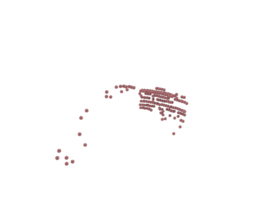
\includegraphics[width=1.75cm,trim={\cropleft cm \croplower cm \cropright cm \cropupper cm},clip]{gdat_kitti_1530_points}
        \end{subfigure}
        \begin{subfigure}[t]{0.48\textwidth}
            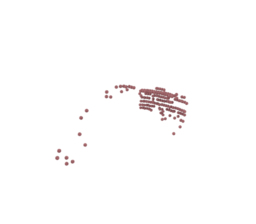
\includegraphics[width=1.75cm,trim={\cropleft cm \croplower cm \cropright cm \cropupper cm},clip]{gdat_kitti_1530_gt}
        \end{subfigure}
        \\
        \begin{subfigure}[t]{0.48\textwidth}
            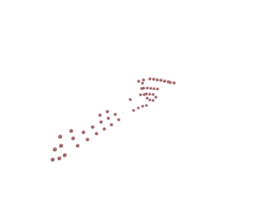
\includegraphics[width=1.75cm,trim={\cropleft cm \croplower cm \cropright cm \cropupper cm},clip]{gdat_kitti_2448_points}
        \end{subfigure}
        \begin{subfigure}[t]{0.48\textwidth}
            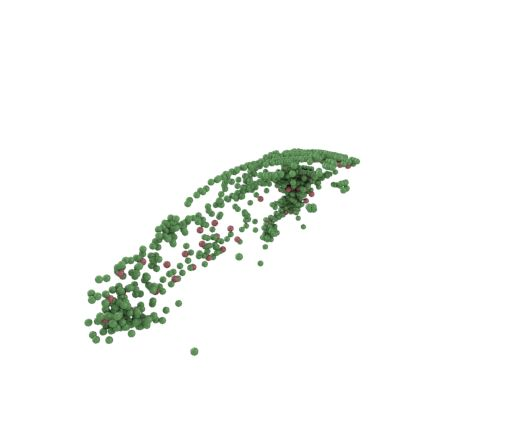
\includegraphics[width=1.75cm,trim={\cropleft cm \croplower cm \cropright cm \cropupper cm},clip]{gdat_kitti_2448_gt}
        \end{subfigure}
        \subcaption{KITTI, Point Clouds}
    \end{subfigure}
    \begin{subfigure}[t]{0.235\textwidth}
        \vspace{0px}\centering
        \begin{subfigure}[t]{0.48\textwidth}
            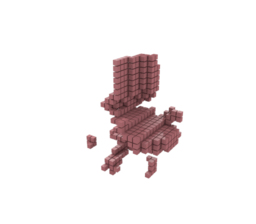
\includegraphics[width=1.75cm,trim={\cropleft cm \croplower cm \cropright cm \cropupper cm},clip]{gdat_yang_chair_1_bin_points}
        \end{subfigure}
        \begin{subfigure}[t]{0.48\textwidth}
            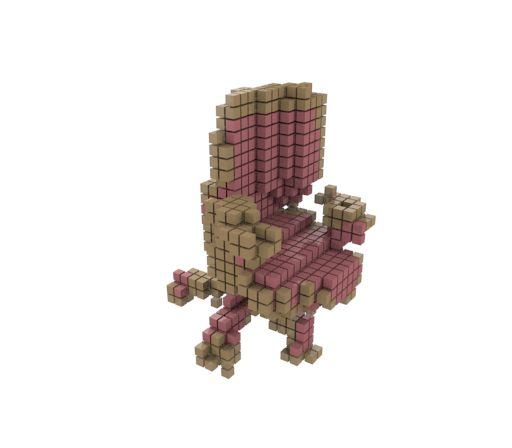
\includegraphics[width=1.75cm,trim={\cropleft cm \croplower cm \cropright cm \cropupper cm},clip]{gdat_yang_chair_1_bin}
        \end{subfigure}
        \\
        \begin{subfigure}[t]{0.48\textwidth}
            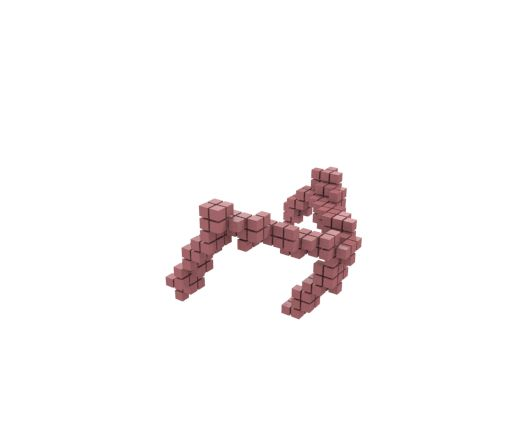
\includegraphics[width=1.75cm,trim={\cropleft cm \croplower cm \cropright cm \cropupper cm},clip]{gdat_yang_table_5_bin_points}
        \end{subfigure}
        \begin{subfigure}[t]{0.48\textwidth}
            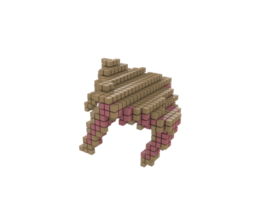
\includegraphics[width=1.75cm,trim={\cropleft cm \croplower cm \cropright cm \cropupper cm},clip]{gdat_yang_table_5_bin}
        \end{subfigure}
        \subcaption{\Kinect, Occupancy Grids}
    \end{subfigure}
    \vspace*{-\figskipcaption px}
	\caption{{{\bf Extracted KITTI and \Kinect Data.} For KITTI, we show observed points in {\color{rred}red} and the accumulated, partial ground truth in {\color{rgreen}green}. Note that for the first example ground truth is not available due to missing past/future observations. For \Kinect, we show observations in {\color{rred}red} and ElasticFusion \citep{Whelan2015RSS} ground truth in {\color{rbeige}beige}. Note that the objects are rotated and not aligned as in ModelNet (\cf \figref{fig:data-shapenet-modelnet}).}}
	\label{fig:data-kitti-yang}
    \vspace*{-\figskipbelow px}
\end{figure}

\boldparagraph{KITTI}
%
We extract observations from KITTI's Velodyne point clouds using the provided ground truth 3D bounding boxes to avoid the inaccuracies of 3D object detectors (train/test split by \cite{Chen2016ARXIV}). As the 3D bounding boxes in KITTI fit very tightly, we first padded them by factor $0.25$ on all sides; afterwards, the observed points are voxelized into voxel grids of size $H \ntimes W \ntimes D = 24 \ntimes 54 \ntimes 24$, $32 \ntimes 72 \ntimes 32$ and $48 \ntimes 108 \ntimes 48$ voxels. To avoid taking points from the street, nearby walls, vegetation or other objects into account, we only consider those points lying within the original (\ie, not padded) bounding box. Finally, free space is computed using ray tracing as described above. We filter all observations to ensure that each observation contains a minimum of $50$ observations. For the bounding boxes in the test set, we additionally generated partial ground truth by accumulating the 3D point clouds of $10$ future and $10$ past frames around each observation. Examples are shown in \figref{fig:data-kitti-yang}.

\boldparagraph{ModelNet}
%
We use ModelNet10, comprising $10$ popular object categories (bathtub, bed, chair, desk, dresser, monitor, night stand, table, toilet) and select, for each category, the first $200$ and $20$ shapes from the provided training and test sets. Then, we follow the pipeline outlined in \figref{fig:data-shapenet-modelnet}, as on ShapeNet, using $10$ random variants per shape. Due to thin structures, however, SDF computation does not work well (especially for low resolution, \eg, $32^3$ voxels). Therefore, we approximate the SDFs using a 3D distance transform on the occupancy grids. Our experiments are conducted at a resolution of $H \ntimes W \ntimes D = 32^3$, $48^3$ and $64^3$ voxels. Given the increased difficulty, we use a resolution of $64^2$, $96^2$ and $128^2$ pixels for the observation generating depth maps. In our experiments, we consider bathtubs, chairs, desks and tables individually, as well as all $10$ categories together (resulting in $100\text{k}$ views overall). For \Kinect, we additionally used a dataset of rotated chairs and tables aligned with \Kinect's ground plane.

\begin{table}[t]
    \vspace*{-\figskipabove px}
    \centering
    {\small
        \begin{tabularx}{0.49\textwidth}{|@{ }X@{ }|@{ }c@{ }|@{ }c@{ }|@{ }c@{ }|@{ }c@{ }|}
            \hline
            & \multicolumn{2}{c@{ }|@{ }}{\bf Synthetic} & \multicolumn{2}{@{ }c@{ }|}{\bf Real}\\
            \hline
            & \clean/-noisy & ModelNet & KITTI & \Kinect\\
            \hline\hline
            \multicolumn{5}{|@{ }c@{ }|}{Training/Test Sets}\\[-2px]
            \multicolumn{5}{|@{ }c@{ }|}{\scriptsize\#Shapes for Shape Prior, \#Views for Shape Inference}\\
            \hline
            \#Shapes & 500/100 & 1000/200& \color{gray}-- & \color{gray}-- \\
            \#Views & 5000/1000 & 10000/2000& 8442/9194 & 30/10\\
            \hline
            \hline
            \multicolumn{5}{|@{ }c@{ }|}{Observed Voxels in \% ({\bf\color{rred}$<5\%$}) \& Resolutions}\\[-2px]
            \multicolumn{5}{|@{ }c@{ }|}{\tiny Low = $24\ntimes54\ntimes24$/$32^3$; Medium = $32\ntimes72\ntimes32$/$48^3$; High = $48\ntimes108\ntimes48$/$64^3$}\\
            \hline
            Low & 7.66/3.86 & 9.71& 6.79 & \bf\color{rred}0.87\\
            Medium & 6.1/\bf\color{rred}2.13 & 8.74& 5.24 & \color{gray}--\\
            High & \bf\color{rred}2.78/\bf\color{rred}0.93 & 8.28& \bf\color{rred}3.44 & \color{gray}--\\
            \hline
        \end{tabularx}
    }
    \vspace*{-\figskipcaption px}
	\caption{{\bf Dataset Statistics.} We report the number of (rotated and scaled) meshes, used as reference shapes, and the resulting number of observations (\ie, views, $10$ per shape). We also report the average fraction of observed voxels, \red{\ie, $\nicefrac{|\{x_i \neq \uk\}|}{HWD}$}. For ModelNet, we exemplarily report statistics for chairs; and for \Kinect, we report statistics for tables.}
	\label{tab:data}
    \vspace*{-\figskipbelow px}
\end{table}

\boldparagraph{\Kinect}
%
Yang \etal provide Kinect scans of various chairs and tables. They provide both single-view observations as well as ground truth from ElasticFusion \citep{Whelan2015RSS} as occupancy grids. However, the ground truth is not fully accurate, and only $40$ views are provided per object category. Still, the objects have been segmented to remove clutter and are appropriate for experiments in conjunction with ModelNet10. Unfortunately, Yang \etal do not provide SDFs; again, we use 3D distance transforms as approximation. Additionally, the observations do not indicate free space and we were required to guess an appropriate ground plane. For our experiments, we use $30$ views for training and $10$ views for testing, see \figref{fig:data-kitti-yang} for examples.